%----------------------------------------------------------
\def\notedate{2021.11.10}
\def\currentauthor{Крехтунова Д.Д. (РК6-73Б)}
%----------------------------------------------------------
\notestatement{rndhpcdbg}{Автоматизированные и автоматические методы отладки, применяемые при реализации сложных вычислительных методов (СВМ), отладка наукоёмкого кода, science code debugging, graph based programming и пр. (первичный обзор литературы)}

%---------------------------------------------------------
\subsubsection{Анализ взвешенных графов вызовов для локализации ошибок программного обеспечения}

Далее представлен материал, являющийся результатом анализа работы \cite{Eichinger2008}.

\paragraph{Проблема}

Обнаружение сбоев, которые приводят к ошибочным результатам с некоторыми, но не со всеми входными данными.

\paragraph{Предложенное решение}

Метод анализа графов вызовов функций с последующим составлением рейтинга методов, которые вероятнее всего содержат ошибку. 

\paragraph{Описание решения}\messnote{Решения чего?}

\textit{Граф вызовов}

Метод основан на анализе графа вызовов. Такой граф отражает структуру вызовов при выполнении конкретной программы. Без какой-либо дополнительной обработки граф вызовов представляет собой упорядоченное дерево с корнем.

\begin{figure}[!ht]
	\centering
	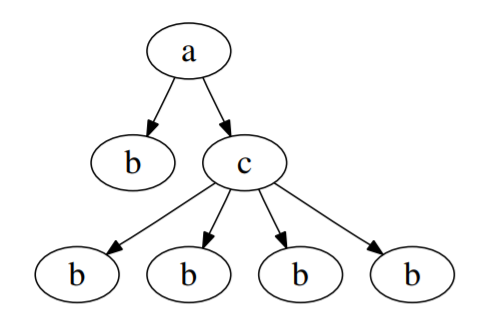
\includegraphics[width=0.3\textwidth]{ResearchNotes/rndhpc_not_dbg_2021_11_10/graph.png}
	\caption{Граф вызовов} 
\end{figure}

Узлами являются сами методы, а гранями -- их вызовы. Метод main() программы обычно является ее корнем, а все методы, вызываемые напрямую, являются ее дочерними элементами.

\textit{Редукция графа}

Трассировка представляется в виде графов вызовов, затем повторяющиеся вызовы методов, вызванные итерациями, удаляются, вместо этого вводятся веса ребер, представляющие частоту вызовов. 

\begin{figure}[!ht]
	\centering
	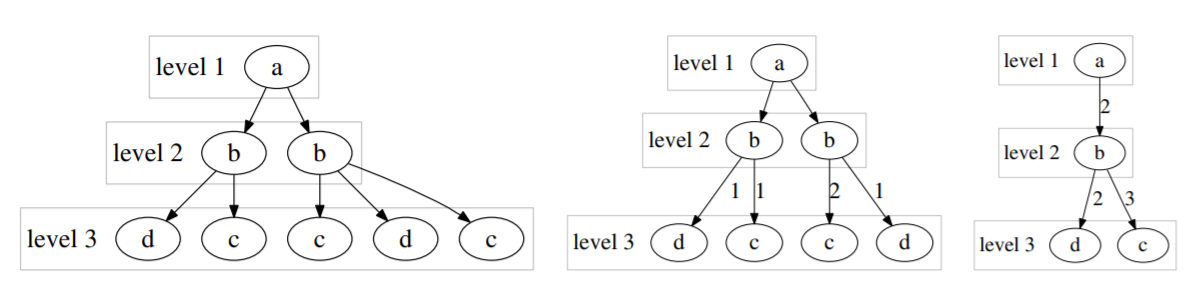
\includegraphics[width=1\textwidth]{ResearchNotes/rndhpc_not_dbg_2021_11_10/reduction.png}
	\caption{Редукция графа вызовов} 
\end{figure}

\textit{Поиск подграфов}

Для поиска подграфов используется фреймворк для ранжирования потенциально ошибочных методов.

После сокращения графов вызовов, полученных от правильного и неудачного выполнения программ, применяется поиск часто встречающихся замкнутых подграфов SG в наборе данных графа G, используя алгоритм CloseGraph. Полученный набор подграфов разделяется на те, которые встречаются при правильном и неудачном выполнении (SGcf), и те, которые возникают только при неудачном выполнении (SGf).

\textit{Анализ}

Два набора подграфов рассматриваются отдельно.

SGcf используется для построения рейтинга на основе различий в весах ребер при правильном и неудачном выполнении. Графы анализируются: применяется алгоритм выбора характеристик на основе энтропии к весам различных ребер для вычисления вероятности вызова метода и вероятности содержания в нем ошибки.

Алгоритм на основе энтропии не может обнаружить ошибки, которые не влияют на частоту вызовов и не учитывает подграфы, которые появляются только в ошибочной версии (SGf).

Поэтому отдельно рассчитывается оценка для методов, содержащихся только в ошибочной версии. Эта оценка - еще одна вероятность наличия ошибки, основанная на частоте вызовов методов при неудачных выполнениях.

Затем вычисляется общая вероятность наличия ошибки для каждого метода. Этот рейтинг дается разработчику программного обеспечения, который выполняет анализ кода подозрительных методов.

% --------------------------------------
\subsubsection{Интегрированная отладка моделей Modelica}

Далее представлен материал, являющийся результатом анализа работы \cite{Pop2014}.

Modelica -- объектно-ориентированный, декларативный язык моделирования сложных систем (в частности, систем, содержащих механические, электрические, электронные, гидравлические, тепловые, энергетические компоненты). 

\paragraph{Проблема}

Из за высокого уровня абстракции и оптимизации компиляторов, обеспечивающих простоту использования, ошибки программирования и моделирования часто трудно обнаружить.

\paragraph{Предложенное решение}

В статье представлена интегрированная среда отладки, сочетающая классическую отладку и специальные техники (для языков основанных на уравнениях) частично основанные на визуализации графов зависимостей.

\paragraph{Описание решения}

На этапе моделирования пользователь обнаруживает ошибку в нанесенных на график результатах, или код моделирования во время выполнения вызывает ошибку.

Отладчик строит интерактивный граф зависимостей (IDG) по отношению к переменной или выражению с неправильным значением.

Узлы в графе состоят из всех уравнений, функций, определений значений параметров и входных данных, которые использовались для вычисления неправильного значения переменной, начиная с известных значений состояний, параметров и времени.

Переменная с ошибочным значением (или которая вообще не может быть вычислена) отображается в корне графа.

Ребра могут быть следующих двух типов.
\begin{itemize}
	\item Ребра зависимости данных: направленные ребра, помеченные переменными или параметрами, которые являются входными данными (используются для вычислений в этом уравнении) или выходными данными (вычисляются из этого уравнения) уравнения, отображаемого в узле.
	\item Исходные ребра: неориентированные ребра, которые связывают узел уравнения с реальной моделью, к которой принадлежит это уравнение.
	ребра, указывающие из сгенерированного исполняемого кода моделирования на исходные уравнения или части уравнений, участвующие в этом коде \messnote{Непонятно}
\end{itemize}

Пользователь может:
\begin{itemize}
	\item Отобразить результаты симуляции, выбрав имя переменной или параметра(названия ребер). График переменной покажется в дополнительном окне. Пользователь может быстро увидеть, имеет ли переменная ошибочное значение.
	\item Отобразить код модели следуя по исходным ребрам.
	\item Вызвать подсистему отладки алгоритмического кода, если пользователь подозревает, что результат переменной, вычисленной в уравнении, содержащем вызов функции, неверен, но уравнение кажется правильным.
\end{itemize}

Используя эти средства интерактивного графа зависимостей, пользователь может проследить за ошибкой от ее проявления до ее источника.

%-------------------------------------------
\subsubsection{Систематические методы отладки для масштабных вычислительных фреймворков высокопроизводительных вычислений}

Далее представлен материал, являющийся результатом анализа работы \cite{Humphrey2014}.

Параллельные вычислительные фреймворки для высокопроизводительных вычислений играют центральную роль в развитии исследований, основанных на моделировании, в науке и технике.

Фреймворк Uintah был создан для решения сложных задач взаимодействия жидких структур с использованием параллельных вычислительных систем.

\paragraph{Проблема}

Поиск и исправление ошибок в параллельных фреймворках, возникающих из-за параллельного характера кода.

\paragraph{Предложенное решение}

В статье описывается подход к отладке крупномасштабных параллельных систем, основанный на различиях в исполнении между рабочими и нерабочими версиями. Подход основывается на трассировке стека вызовов.

Исследование проводилось для вычислительной платформы Uintah Computational Framework.

\paragraph{Описание решения}

Так как количество трассировок стека, которые можно получить при выполнении программы, может быть большим, для лучшего понимания используются графы, которые могут сжать несколько миллионов трассировок стека в одну управляемую фигуру. Метод основан на получении объединенных графов трассировки стека (CSTG). 

Хотя сбор и анализ трассировки стека ранее изучались в контексте инструментов и подходов, их внимание не было сосредоточено на кросс-версии (дельта) отладке.

\begin{figure}[h]
	\centering
	\begin{minipage}{0.45\textwidth}
	\centering
	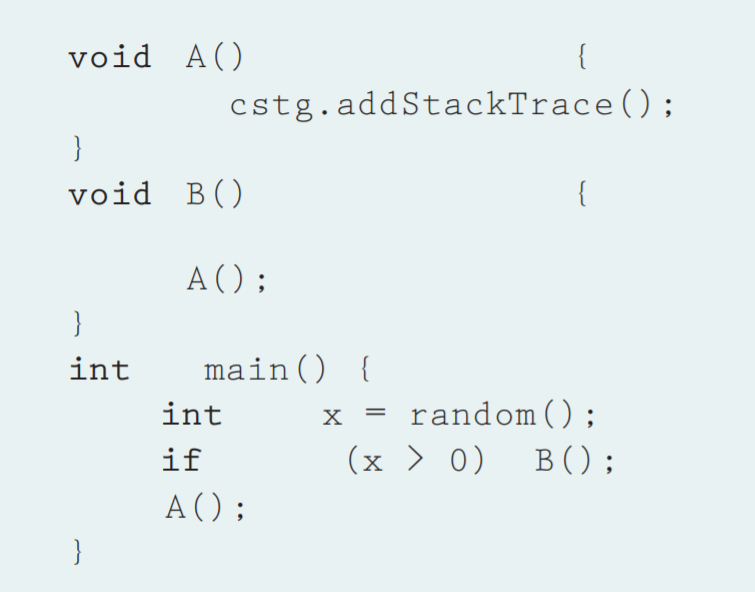
\includegraphics[width=1\textwidth]{ResearchNotes/rndhpc_not_dbg_2021_11_10/prog_ex.png}
	\end{minipage}
	\begin{minipage}{0.5\textwidth}
	\centering
	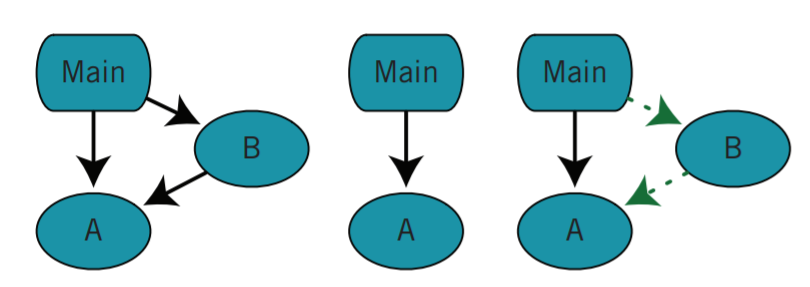
\includegraphics[width=1\textwidth]{ResearchNotes/rndhpc_not_dbg_2021_11_10/cstg.png}
	\end{minipage}
	\caption{Пример построения CSTG} 
\end{figure}

CSTG не записывают каждую активацию функции, а только те, что в трассировках стека ведут к интересующей функции (функциям), выбранной пользователем. Каждый узел CSTG представляет все активации конкретного вызова функции. Помимо имен функций, узлы CSTG также помечаются уникальными идентификаторами вызова. Грани представляют собой вызовы между функциями. 

\begin{figure}[h]
	\centering
	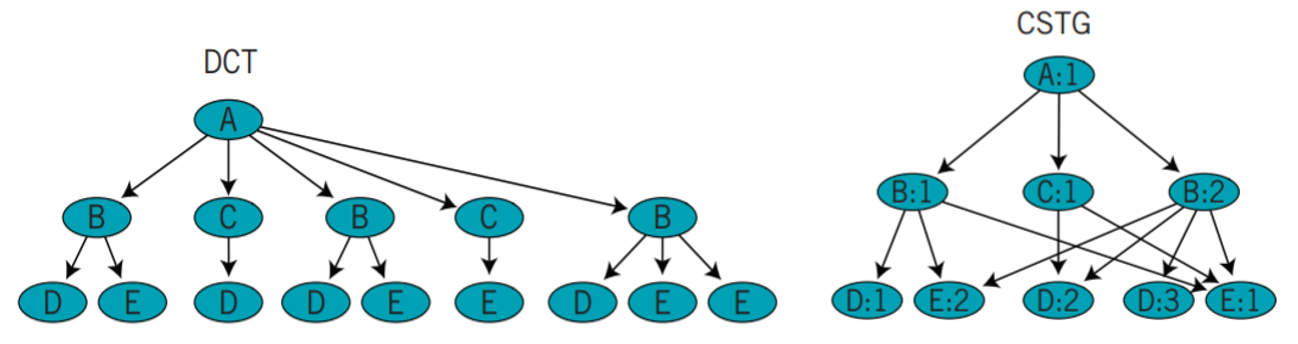
\includegraphics[width=1\textwidth]{ResearchNotes/rndhpc_not_dbg_2021_11_10/cstg2.png}
	\caption{CSTG} 
\end{figure}

Пользователю необходимо вставить в интересующие функции вызовы cstg.addStackTrace(). Инструмент CSTG автоматически запускает тестируемый пример с использованием различных сценариев, создает графы и помогает пользователям увидеть существенные различия между сценариями. Сама ошибка обычно обнаруживается и подтверждается с помощью традиционного отладчика, при этом дельта-группы CSTG наводят на место возникновения ошибки.

%----------------------------
\subsubsection{Ориентированный на данные фреймворк для отладки параллельных приложений}

Далее представлен материал, являющийся результатом анализа работы \cite{Dinh2013}.

\paragraph{Проблема}

Обнаружение ошибок в крупномасштабных научных приложениях, работающих на сотнях тысяч вычислительных ядер.

Неэффективность параллельных отладчиков для отладки пета-масштабных приложений.

\paragraph{Предложенное решение}

В этом исследовании представлена реализация фреймворка для отладки, ориентированного на данные, в котором в качестве основы используются утверждения. Подход, ориентированный на данные можно использовать для повышения производительности параллельных отладчиков. 

Метод, представленный в статье основан на параллельном отладчике Guard, который поддерживает тип утверждения во время отладки, называемые сравнительные утверждения. 

\paragraph{Описание решения}

Утверждение -- это утверждение о предполагаемом поведении компонента системы, которое должно быть проверено во время выполнения. В программировании программист определяет утверждение, чтобы гарантировать определенное состояние программы во время выполнения.

Пользователь делает заявления о содержимом структур данных, затем отладчик проверяет достоверность этих утверждений.

В следующем списке показаны примеры утверждений, которые можно использовать для обнаружения ошибок во время выполнения:

\begin{itemize}
	\item «Содержимое этого массива всегда должно быть положительным».
	\item «Сумма содержимого этого массива всегда должна быть меньше постоянной границы».
	\item «Значение в этом скаляре всегда должно быть больше, чем значение в другом скаляре».
	\item «Содержимое этого массива всегда должно быть таким же, как содержимое другого массива». 
\end{itemize}

В работе используются два новых шаблона утверждений помимо сравнительных: общие специальные утверждения и статистические утверждения.

\textit{Общие специальные} утверждения позволяют использовать простые арифметические и булевы операции.

\begin{figure}[h]
	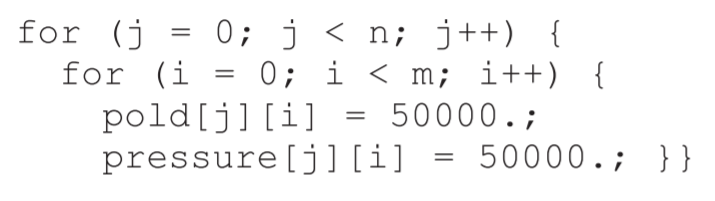
\includegraphics[width=0.5\textwidth]{ResearchNotes/rndhpc_not_dbg_2021_11_10/data_prog.png}
\end{figure}

Например, учитывая следующий фрагмент кода из исходного файла init.c и предполагая, что код вызывается с набором процессов \$a, можно рассмотреть следующее утверждение:

\begin{figure}[h]
	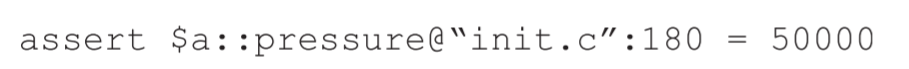
\includegraphics[width=0.6\textwidth]{ResearchNotes/rndhpc_not_dbg_2021_11_10/assert1.png}
\end{figure}

Это утверждение гарантирует, что каждый элемент в структуре данных набора процессов \$a равен 50 000 в строке 180 исходного файла init.c

Соответственно, \textit{сравнительные утверждения} позволяют сравнивать две отдельные структуры данных во время выполнения.

Следующее утверждение сравнивает данные из big_var в \$a в строке 4300 исходного файла ref.c с large_var в \$b в строке 4300 исходного файла sus.c.

\begin{figure}[h]
	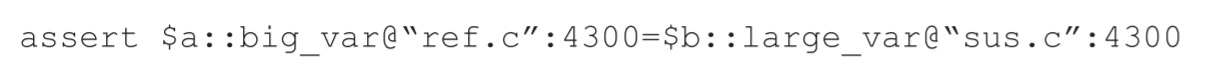
\includegraphics[width=0.8\textwidth]{ResearchNotes/rndhpc_not_dbg_2021_11_10/assert2.png}
\end{figure}

\textit{Статистические утверждения} - это определяемый пользователем предикаты, состоящие из двух моделей данных в форме либо статистических примитивов (средние значения, значения стандартного отклонения), либо функциональных моделей (гистограммы, функции плотности)

Статистические утверждения позволяют пользователю сравнивать информацию о шаблонах данных между двумя структурами данных, тогда как более ранние утверждения требовали сравнения точных значений.

Например, можно утверждать, что среднее значение большого набора данных находится между определенными границами до или после вызова функции или что количество элементов в массиве должно находиться в определенном диапазоне.

%-------------------------
\subsubsection{Определение степени и источников недетерминизма в приложениях MPI с помощью ядер графов}

Далее представлен материал, являющийся результатом анализа работы \cite{Chapp2021}.

\paragraph{Проблема}

Выявление причин сбоев воспроизводимости в приложениях на экзафлопсных платформах.

Крупномасштабные приложения MPI обычно принимают гибкие решения во время выполнения том порядке, в котором процессы обмениваются данными, чтобы улучшить свою производительность. Следовательно, недетерминированные коммуникативные модели стали особенностью этих научных приложений в системах высокопроизводительных вычислений.

Недетерминизм мешает разработчикам отслеживать вариации выполнения программы для отладки. Также сложно воспроизвести результаты при повторных запусках, что затрудняет доверие к научным результатам.

\paragraph{Предложенное решение}

Фреймворк для определения источников недетерминизма с использованием графов событий. 

\paragraph{Описание решения}

Параллельное выполнение программы моделируется в виде ориентированных графов событий, ядра графов используются, чтобы охарактеризовать изменения межпроцессного взаимодействия от запуска к запуску. Ядра могут количественно определять тип и степень недетерминизма, присутствующего в моделях коммуникации MPI.

Фреймворк позволяет найти первопричины недетерминизма в исходном коде без знания коммуникативных паттернов приложения.

Платформа моделирует недетерминизм в следующие три этапа. 

\paragraph{Этап первый. Сбор трассировки выполнения.} Фреймворк фиксирует трассировку нескольких выполнений недетерминированного приложения с помощью двух модулей трассировки: CSMPI (фиксирует стек вызововов, связанных с вызовами функций MPI) и DUMPI (фиксирует порядок отправляемых и получаемых сообщений для каждого процесса MPI).

Для каждого выполнения приложения фреймворк генерирует один файл трассировки CSMPI и один файл трассировки DUMPI для каждого процесса MPI (или ранга). Файлы трассировки впоследствии загружаются конструктором графа событий для восстановления порядка сообщений выполнения.

\paragraph{Этап второй. Построение модели графа событий.} На втором этапе фреймворк моделирует выполнение недетерминированного приложения в виде ориентированного ациклического графа (DAG), используя файлы трассировки, созданные на первом этапе.

Здесь вершины представляют собой связи point-to-point, такие как отправка и получение сообщения, а направленные ребра представляют отношения между этими событиями. Модели межпроцессного взаимодействия этой формы обычно называются графами событий.

\begin{figure}[h]
	\centering
	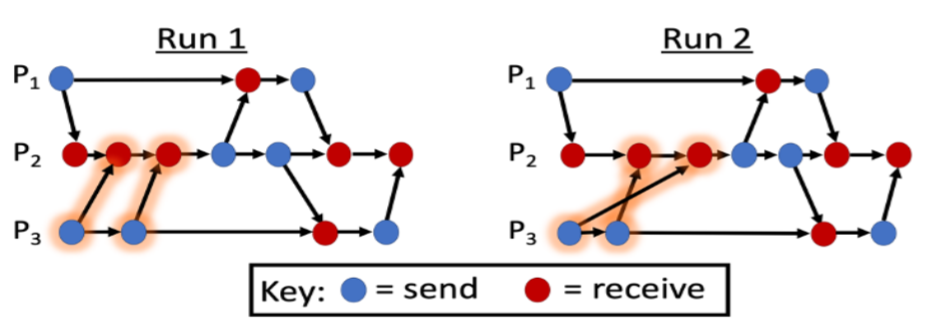
\includegraphics[width=0.7\textwidth]{ResearchNotes/rndhpc_not_dbg_2021_11_10/dga.png}
	\caption{DGA} 
\end{figure}

Затем используются ядра графов для количественной оценки (несходства) графов событий, тем самым количественно оценивая степень проявления недетерминированности в приложении.

Ядра графов представляют собой семейство методов для измерения структурного сходства графов. 

Простыми словами, ядро графа можно рассматривать как функцию, которая подсчитывает совпадающие подструктуры (например, поддеревья) двух входных графов, как показано на рис.~\ref{lab.rndhpc2021.11.10.010}, сопоставляя пары графов со скалярами, которые количественно определяют, насколько они похожи.

\begin{figure}[h]
	\centering
	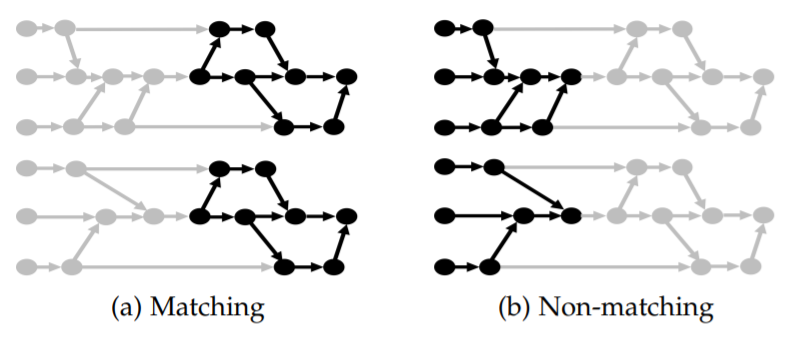
\includegraphics[width=0.6\textwidth]{ResearchNotes/rndhpc_not_dbg_2021_11_10/graph_comp.png}
	\caption{Сравнение двух графов}\label{lab.rndhpc2021.11.10.010}
\end{figure}

\paragraph{Этап третий. Анализ графа событий.} На последнем этапе анализ графа событий позволяет ученым количественно оценить недетерминированность многократного выполнения приложения MPI без каких-либо знаний о коммуникативных моделях приложения MPI.

%----------------------------------------------------------
% Атрибуты задачи
\noteattributes{}
%----------------------------------------------------------

